%%%%%%%%%%%%%%%%%%%%%%%%%%%%%%%%%%%%%%%%%%%%%%%%
% COPYRIGHT: (C) 2012-2015 FAU FabLab and others
% CC-BY-SA 3.0
% EXCEPT for the "Betriebsanweisung" pages!
%%%%%%%%%%%%%%%%%%%%%%%%%%%%%%%%%%%%%%%%%%%%%%%%


\newcommand{\basedir}{fablab-document} % Pfad zur Dokumentenvorlage
\documentclass{\basedir/fablab-document}

\usepackage{booktabs} % für Tabellen: fancy \addlinespace und besondere Querlinien 
\usepackage{pdfpages} % für \includepdf

\usepackage[colorinlistoftodos,prependcaption]{todonotes}
\presetkeys%
    {todonotes}%
    {inline,backgroundcolor=red}{}
\newcommand{\todoUnwichtig}[1]{\textbf{TODO: #1} }
\renewcommand{\texteuro}{\euro}
%\newcommand{\todo}[1]{\textbf{\color{red}{TODO: #1}}}
\newcommand{\pfeil}{\ensuremath{\rightarrow}}
\newcommand{\kommando}[1]{\texttt{#1}}
\newcommand{\tabitem}{~~\llap{\textbullet}~~}
\newcommand{\mcc}[1]{\multicolumn{2}{c}{#1}}
\renewcaptionname{ngerman}{\tablename}{Tab.}

\hyphenation{%
	Reit-stock-auf-nah-me
	Schnell-wech-sel-halt-er
	}

% \linespread{1.2}

\fancyhead[C]{\textbf{\color{red}{TODO: unfertig!}}}
\date{2015}
\author{kontakt@fablab.fau.de}
\title{Einweisung Drehbank}

\begin{document}

\listoftodos

\tableofcontents

\newpage



\section{Einweisungsstufen}

\todo{Abgleich mit Einweisungsliste, zur Zeit inkonsistent bezüglich beaufsichtigter Benutzung Handbetrieb. Möglichkeit Sonder-Einweisung erwähnen}

\begin{enumerate}
 \item Ohne eine unterschriebene Grund-Einweisung in diese Regeln darf die Drehbank garnicht benutzt werden, d.\,h. du darfst dann nichts selber an und in der Drehbank tun.
 \item Mit Grund-Einweisung bist du zunächst \enquote{Fahrschüler} und darfst den Auftrag zwar selber vorbereiten (Werkstück ein- und ausspannen, Drehbank säubern), \textbf{die Steuerung aber nicht selbstständig bedienen.} 

       Ein Benutzer, der die Drehbank selbstständig benutzen darf, prüft dann, ob dein Auftrag keine gefährlichen Fehler enthält, und führt dann als \enquote{Fahrlehrer} gemeinsam mit dir die Arbeit durch.

 Die Bedienung der Steuersoftware (Verfahren, Antasten, Starten, Fortsetzen nach Pause, \dots) darf dabei nur unter ständiger Aufsicht durch den Experten erfolgen!
 \item Sobald du genug Erfahrung und Routine hast und das entsprechend dokumentiert ist (mehrere Werkstücke selbstständig unter Aufsicht gefertigt, dies über einen größeren Zeitraum verteilt), wird dir die schriftliche Erlaubnis erteilt, den CNC-Betrieb ohne Aufsicht zu benutzen. Dabei sollen verschiedene Bearbeitungsarten und Werkzeuge verwendet worden sein.
 \item  \textbf{Für die Benutzung des Handbetriebs ist eine zusätzliche schriftliche Erlaubnis nötig!} Es gelten dabei weitere Vorschriften, siehe Kapitel \ref{handdrehen}.
\end{enumerate}


\newpage
\section{Grundlagen}

Ein denkender Bediener wird generell bei allen Beschreibungen dieses Dokuments vorausgesetzt. Eine Drehmaschine ist ein gefährliches Werkzeug, deren sichere Bedienung unbedingt notwendig ist um schwere Unfälle zu vermeiden.

\subsection{Begriffserklärung}
\begin{tabular}{p{0.15\textwidth} p{0.8\textwidth}}
Achsen 				& Z in Richtung der Drehachse (vom Futter weg = positiv), X senkrecht horizontal zur Drehachse (nach vorne, auf den Bediener zu = positiv) \\
Drehmeißel 		& Komplettes Teil aus Wendeplatte und Wendeplattenhalter. Ist in einem Schnell\-wechsel\-halter eingespannt und darf nicht verändert werden. \\
Körnerspitze 	& Die mitlaufende Körnerspitze steckt anstelle des Bohrfutters in der Aufnahme des Reitstocks. Wird zum Gegenspannen von langen Werkstücken verwendet. Festdrehen, bis die Körnerspitze dauerhaft mitdreht, dann nicht mehr fester machen. Genaue Erklärung in Kapitel \ref{handdrehen:gegenspannen}. \\
Nullpunkte 		& Z i.d.R. beim rechten oder linken Rand des Werkstücks, X in der Drehmitte \\
Reitstock 		& Gegenlager auf der rechten Seite der Hauptachse. Wird verwendet um lange Werkstücke gegenzuspannen. \\
Spannfutter 	& Auf der Hauptspindel befestigt. Haltevorrichtung mit 3 bis 4 Backen, welche das Werkstück aufnehmen und festklemmen. \\
Wendeplatte 	& Das kleine, aus Hartmetall gefertigte Teil, das schließlich das Material zerspant. Brüchig aber sehr hart. Die Kanten können leicht brechen, wenn sie überlastet werden oder Stöße abbekommen. \\
\end{tabular}

\subsection{Zerspanung}
\subsubsection{Was ist Drehen?}
Drehen ist ein zerspanender Prozess, bei dem ein fest eingespanntes Werkzeug (Drehmeißel) am sich drehenden Werkstück entlanggeführt wird.
Der Drehmeißel hat eine geometrisch bestimmte Schneide aus Schnellarbeitsstahl (HSS) oder Wendeschneidplatten aus Vollhartmetall (VHM) und wird quer zur Drehrichtung bewegt.
Daraus ergibt sich eine kreisförmige Schnittbewegung und es entstehen rotationssymtrische Werkstücke.

\newpage
\subsubsection{Drehmeißel}
Ein Drehmeißel besteht aus einem Werkzeugschaft, welcher fest in der Aufnahme befestigt ist. Am vorderen Ende befinden sich die Haupt- und Nebenschneide durch welche das Material
abgetragen wird.
\begin{figure}[ht]
\centering
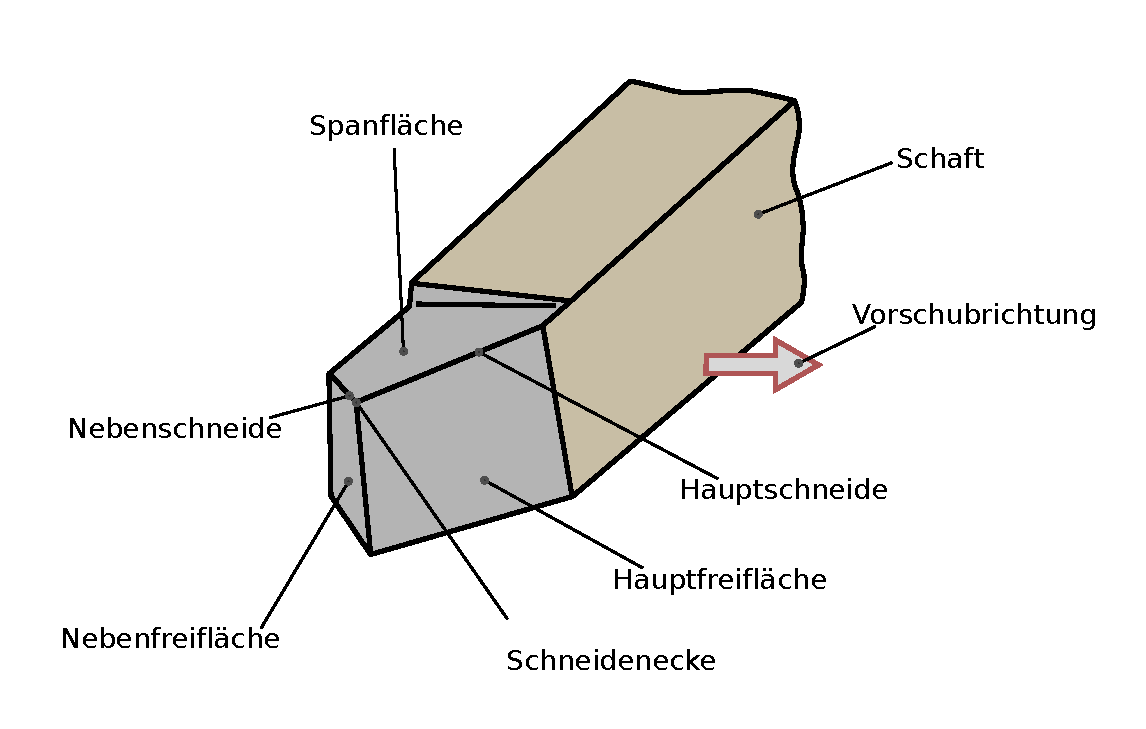
\includegraphics[width = 0.75\linewidth]{img/drehmeissel}
\caption{Flächen am Drehmeißel. Autor: \href{http://commons.wikimedia.org/wiki/File:Flaechen_am_Schneidkeil.svg}{David W.}, Lizenz \href{http://creativecommons.org/licenses/by-sa/2.5}{CC-BY-SA 2.5}}
\end{figure}

\subsubsection{Spannfutter}

Es gibt zwei verschiedene Spannfutter, eines mit 3 Backen und eines mit 4 Backen. Das Spannfutter wird mit dem entsprechenden Schlüssel an der Seite auf und zu gedreht. Beim Spannen ist das mit \emph{0} markierte Loch zu verwenden.

Es gibt im Grunde keine feste Regel nach der das Futter gewählt werden kann, jedoch gibt es einige Erfahrungswerte:
\begin{itemize} 
\item Rundmaterial im Dreibackenfutter spannen
\item Beim Drehen von Passungen kann das Vierbackenfutter von Vorteil sein (Stichwort \enquote{Dreibogengleichdick})
\item 6-Kant-Material ausschließlich im Dreibackenfutter
\item Objekte mit quadratischem Querschnitt ausschließlich im Vierbackenfutter
\end{itemize}

Spannfutter haben einen definierten maximalen Spanndurchmesser, der üblicherweise kleiner als die maximale Backenöffnung ist. Dieser Durchmesser ist unbedingt zu beachten, es besteht die Gefahr von Desintegration im laufenden Betrieb.
\todo{Wie groß ist dieser Maximaldurchmesser?}
\todo{Überschneidung mit Abschnitt Rohmaterial einspannen -- umsortieren?}

\subsubsection{Spannfutterwechsel}

Achtung das Spannfutter ist schwer! Lass dir am Besten von jemandem helfen. Achte unbedingt auf Sauberkeit, insbesondere Spanfreiheit!
\begin{itemize}
\item Maul- und Imbusschlüsselsatz holen
\item Abdeckhaube wegklappen
\item Am Besten etwas unterlegen, damit es nicht herunterfällt
\item Schrauben auf der Rückseite des Futters lösen und dabei festhalten 
\item Nach dem Lösen vorsichtig herausnehmen, ggf. vorsichtig mit dem Schonhammer nachhelfen
\item Hinten am Futter befindet sich ein Adapter für die Aufnahme, dieser muss nun mit einem Innensechskant abgeschraubt werden
\item Den Adapter auf das andere Futter montieren
\item Das neue Futter wieder vorsichtig einsetzen und beim Festschrauben darauf achten, dass es nicht verkantet
\item Das ausgebaute Futter vor dem Einlagern säubern und ölen
\end{itemize}

\subsubsection{Spannbacken}

Es gibt Innen- und Außenspannbacken.
Innenspannbacken werden zum Spannen von Innenradien wie z.\,B. Bohrungen sowie von kleinen bis mittelgrossen Aussenradien verwendet. Innenspannbacken haben dazu sowohl innere als auch äussere Spannflächen.

Außenspannbacken kommen hingegen ausschliesslich beim Spannen auf Außenflächen zum Einsatz.
Wichtig: Sechskantmaterial immer mit den Innenbacken spannen.

\todo{Bilder}

\subsubsection{Spannbackenwechsel}
\label{zerspanung:spannbackenwechsel}
Achte \emph{unbedingt} auf Sauberkeit!
 
Die Spannbacken befinden sich in der Schublade unter der Drehbank.
Um die alten Spannbacken zu entfernen muss man diese mit dem Spannfutterschlüssel herausdrehen.
Die Spannbacke mit der Nummer 3 löst sich zuerst, danach die Nummer 2 und 1.
Achte dabei darauf, dass die Spannbacken nicht herausfallen.

Das Einsetzen der neuen Spannbacken beginnt mit der Nummer 1.
Unbedingt darauf achten, dass die Spannbacke Nummer 1 auch an der Postion 1 des Spannfutters eingesetzt wird!
Achte darauf keinen Schmutz oder Späne ins Futter zu bringen. Hierzu vor dem Einbau die Spannbacken vorsichtig mit Druckluft ausblasen.

Das Prinzip der Spannbackenbefestigung ist eine Spirale, die in die Nuten der Spannbacken greift.
Drehe solange den Spannfutterschlüssel, bis der Beginn der Spirale bei Spannbacken 1 zu sehen ist.
Dann drehe ein kleines Stück zurück und schiebe die Spannbacke bis zum Anschlag in die Nut und drehe mit dem Spannfutterschlüssel ein wenig weiter.
Das Vorgehen wiederholt man bei den Spannbacken 2 und 3.

Zum Ende das Futter einmal vollständig zudrehen.
Wenn nun die Spannbacken sauber schließen ist alles richtig gemacht.
Wenn eine Spannbacke jedoch zu früh oder zu spät in der Mitte ankommt, wurde diese falsch eingesetzt.
In diesem Fall müssen alle Spannbacken wieder ausgebaut und die Prozedur komplett wiederholt werden.

Die ausgebauten Spannbacken säubern, ölen und wieder aufräumen.

\subsubsection{Kühlschmierstoff}

Das Kühlschmiermittel besteht aus einer Öl-Wasser-Emulsion.
Die Aufgabe des Kühlschmierstoffes (KSS) besteht darin den Schneidvorgang zu kühlen (Wasser) und zu schmieren (Öl).
Aufgrund der Zusätze und der entfettenden Wirkung des Emulgators sollte der Hautkontakt vermieden werden.
Bei Augenkontakt sofort mit reichlich Wasser ausspülen und gelegentlich die oberen und unteren Augenlieder anheben.
Anschließend ist ein Augenarzt aufzusuchen.

\subsubsection{Drehbank}
Unsere Drehbank besteht aus Hauptspindel mit Futterschutzhaube, Reitstock, Werkzeughalter, Kühlmittelpumpe, CNC-Steuerung und Einhausung mit Kunststoffschutzhaube.
\begin{figure}[ht]
\centering
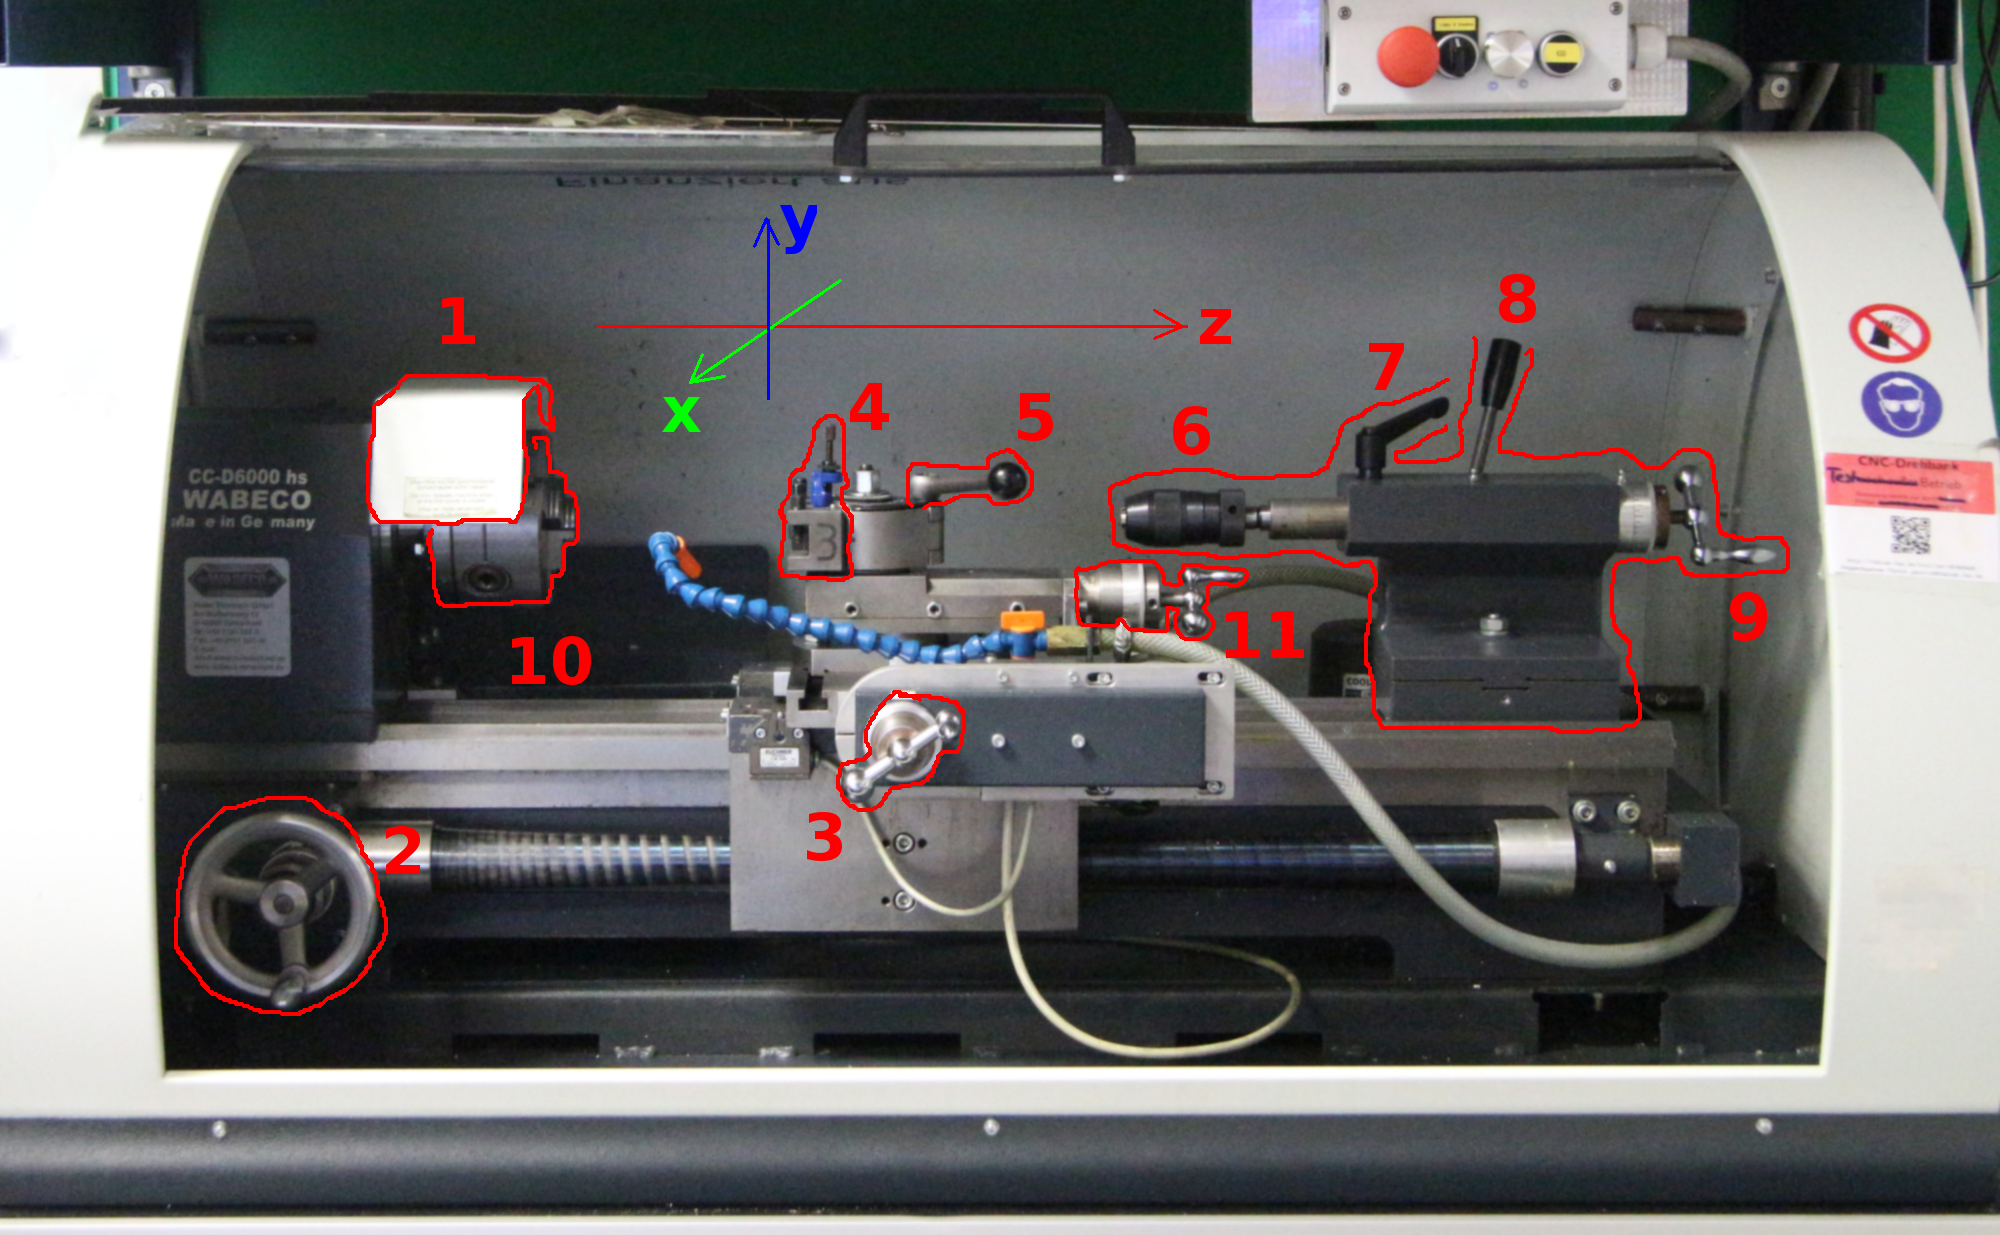
\includegraphics[width = 0.9\linewidth]{img/drehbank-uebersicht-beschreibung} \\
\caption{Bezeichnungen der Maschinenteile: 1: Futterschutzhaube; 2: Handverstellrad Z-Achse; 3: Handverstellrad X-Achse; 4: Werkzeughalter; Schnellspan-; 5: Feststellhebel Schnellspanhalterung; 6: Bohrfutter, hier kann stattdessen auch die mitlaufende Körnerspitze eingesetzt werden; 7: Feststellhebel Feineinstellung Reitstock; 8: Feststellhebel Grob/Verschiebung Reitstock; 9: Feineinstellung Reitstock; 10: Spannfutter; 11: Einstellung Planschlitten(?). Das blaue verstellbare Rohr zwischen 3 und 4 ist die KSS-Düse. Die am Koordinatensystem eingezeichneten Pfeilspitzen zeigen jeweils in positive Koordinatenrichtung. Der Koordinatennullpunkt ist einstellbar und im allgemeinen nicht an der dargestellten Stelle.}
\end{figure}


\subsubsection{Drehprozess}
\begin{tabular}{lll}
    Schnittgeschw. in $\frac{m}{min}$ 					& $v_c = \pi \cdot d \cdot n $ 			& Geschwindigkeit mit der das Material auf den Drehmeißel trifft 	\\ 
																								&																		& Material- und geometrieabhängiger Wert siehe \ref{Schnittwerte} \\ \addlinespace
		Drehzahl in $\frac{1}{min}$ 								& $ n = \frac{v_c}{\pi \cdot d} $		& Drehzahl der Hauptspindel, ergibt sich aus $v_c$								\\ \addlinespace
		spezifischer Vorschub in $mm$ 														& $ f_z $  													& Materialstärke welche pro Umdrehung abgetragen wird 						\\
																								&																		& Material- und geometrieabhängiger Wert siehe \ref{Schnittwerte} \\ \addlinespace
		Vorschubgeschw. in $\frac{mm}{min}$ 				& $ v_f = n \cdot f_z $ 						& Geschwindigkeit mit der der Drehmeißel verfährt			 						\\ \addlinespace
		Zustellung in $mm$ 													& $ h  $  													& Materialstärke welche auf einmal vom Radius weggenommen wird		\\
																								&																		& Material- und prozessabhängiger Wert siehe \ref{Schnittwerte} 	\\ \addlinespace
\end{tabular}

\begin{figure}[ht]
\centering
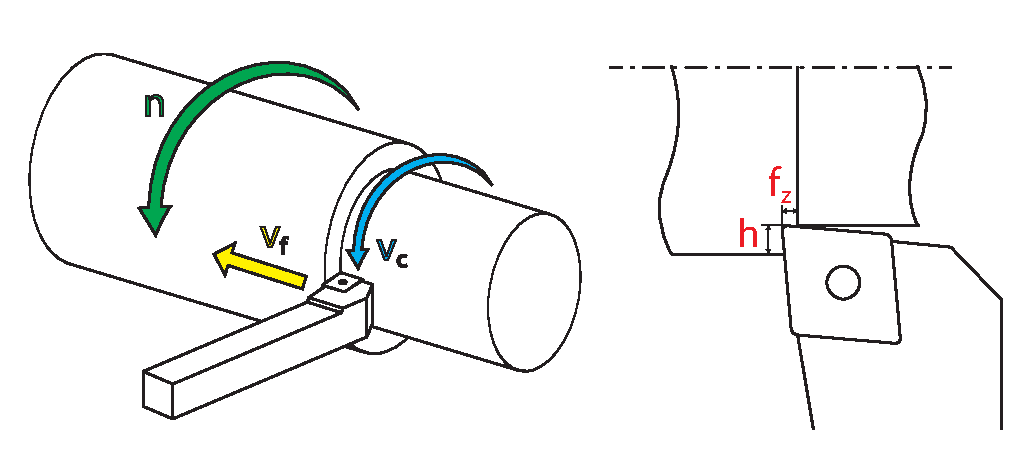
\includegraphics[width = 0.9\linewidth]{img/drehprozess}
\caption{Größen beim Drehprozess.\\Autor: Michael Jäger, selbst erstellt nach Folien des FAPS, FAU Erlangen}
\end{figure}


\subsubsection{Spanformen}
Die Spanbildung bzw. Spanform ist sehr wichtig für die erreichbare Oberflächengüte und hängt sowohl vom Material, als auch von den Prozessparametern ab. \\[1em]
\begin{tabular}{ll}
    Fließspan		& \tabitem kontinuierliche, fließende Spanbildung (Achtung! Verhedderungsgefahr)													\\ 
								&	\tabitem großer Spanwinkel, hohe Schnittgeschwindigkeit, $v_c > 80 \frac{m}{min} $											\\
								&	\tabitem Spanen gut plastisch verformbarer Werkstoffe, z.\,B. Aluminium																		\\
								&	\tabitem hohe Oberflächengüte																																						\\ \addlinespace
    Scherspan		& \tabitem lamellenförmig abgetrennte Spannteilchen, verschweißen wieder in der Scherzone									\\ 
								&	\tabitem mittlere Spanwinkel und Schnittgeschwindigkeit, $20 \frac{m}{min} < v_c < 80 \frac{m}{min} $		\\
								&	\tabitem Spanen zäherer Werkstoffe, z.\,B. Stahl mittlerer Festigkeit 																		\\
								&	\tabitem mittlere Oberflächengüte																																				\\ \addlinespace
    Reißspan		& \tabitem Herausreißen einzelner Spanteile aus dem Werkstoff																							\\ 
								&	\tabitem kleiner Spanwinkel, niedrige Schnittgeschwindigkeit, $v_c < 20 \frac{m}{min} $									\\
								&	\tabitem Spanen spröder Werkstoffe, z.\,B. Gusseisen, Hartguss, Kupfer-Zink-Legierungen, Messing					\\
								&	\tabitem raue Werkstückoberfläche																																				\\ \addlinespace
\end{tabular}
\begin{figure}[ht]
\centering
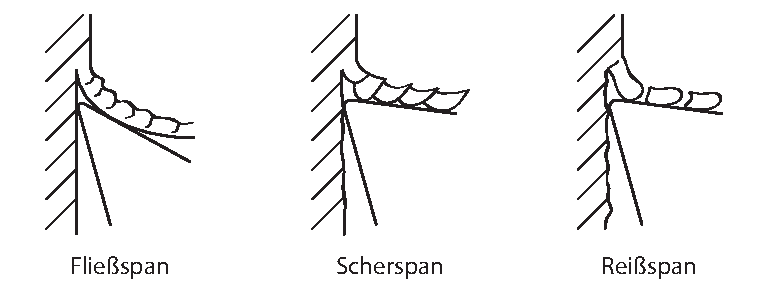
\includegraphics[width = \linewidth]{img/spanformen}
\caption{Spanformen. Autor: Michael Jäger, selbst erstellt nach Folien des FAPS, FAU Erlangen}
\end{figure}

\subsubsection{Schnittwerte}
\label{Schnittwerte}
Der Vorschub ist in den Datenblättern der Werkzeuge meist als spezifischer Vorschub angegeben (mm pro Umdrehung) und muss entsprechend mit der Drehzahl multipliziert werden.
In der Praxis nimmt man die ungefähre Größenordnung aus der Tabelle und probiert.

Zu niedriger Vorschub führt dazu, dass zu wenig Span abgenommen wird und das Werkstück eher gerieben als zerspant wird.
Das setzt das Werkzeug zu und verschlechtert die Schneide.
Zu hoher Vorschub hingegen belastet Werkzeug und Maschine unnötig,
führt zu erhöhtem Verschleiß und kann die Spindel überlasten, wodurch die Drehzahl einbricht.

Die Zustellung ist immer als Absolutwert angegeben.
Bei der Zustellung sind die Auswirkungen ähnlich wie beim Vorschub.

Bei zu großer Zustellung können Stücke aus dem Material ausreißen oder das Werkstück aus dem Futter
springen und den Bediener schwer verletzen!

Dabei gilt, dass der Vorschub beim sogenannten Schruppen höher ist als beim Schlichten.
Schruppen dient in erster Linie dem Abtrag von Material und erzeugt in der Regel eine rauhe Oberfläche mit Riefen.
Schlichten hingegen ist die finale Bearbeitung auf das endgültige Maß in meist einem Durchgang.
Die Oberfläche wird dabei wesentlich feiner. 

\begin{table}
\setlength{\tabcolsep}{0.5em}
\begin{tabular}{rcccccc}
  \textbf{Werkstoff}  & \mcc{$\mathbf{v_c} \textrm{ in } \frac{m}{min} $} & \mcc{$\mathbf{f_z} \textrm{ in } mm$} & \mcc{$\mathbf{h_{max}} \textrm{ in } mm$} \\ \addlinespace \toprule
															& Schruppen 	& Schlichten 	& Schruppen 	& Schlichten 	& Schruppen 	& Schlichten		\\ \toprule
  unleg. Stahl (0,15\% C)			& 370 	& 420  	& 0.17 	& 0.12	& 3.5 	& 1.0 	\\
  unleg. Stahl (0,45\% C)			& 280 	& 315  	& 0.20 	& 0.15	& 3.5 	& 1.0 	\\
  unleg. Stahl (0,55\% C)			& 255 	& 295  	& 0.20 	& 0.15	& 3.5 	& 1.0 	\\
	leg. Stahl									& 345 	& 380  	& 0.17 	& 0.12	& 3.5 	& 1.0 	\\
	leg. Stahl (Cr-Mo)					& 255 	& 295  	& 0.20 	& 0.15	& 3.5 	& 1.0 	\\	
	leg. Stahl (Ni-Cr-Mo)				& 250 	& 285  	& 0.20 	& 0.15	& 3.5 	& 1.0 	\\
	Wälzlagerstahl							& 255 	& 295  	& 0.20 	& 0.15	& 3.5 	& 1.0 	\\
	unleg. Werkzeugstahl				& 255 	& 295  	& 0.20 	& 0.15	& 3.5 	& 1.0 	\\	
	leg. Werkzeugstahl					& 250 	& 285  	& 0.20 	& 0.15	& 3.5 	& 1.0 	\\	
	Schnellarbeitsstahl					& 145 	& 210  	& 0.15 	& 0.10	& 3.5 	& 1.0 	\\	
	Kaltarbeitsstahl						& 195 	& 225  	& 0.18 	& 0.14	& 3.5 	& 1.0 	\\	
	gehärteter Stahl ($<$40HRC)	& 120 	& 120  	& 0.12 	& 0.10	& 3.5 	& 1.0 	\\	
	hochleg. Stahl	(mart./fer.)& 195 	& 270  	& 0.17 	& 0.12	& 3.5 	& 1.0 	\\
	hochleg. Stahl	(aust.)			& 160 	& 220  	& 0.17 	& 0.12	& 3.5 	& 1.0 	\\
	Superlegierung (Ni)					& 50	 	& 60  	& 0.15 	& 0.10	& 3.5 	& 1.0 	\\
	Titan												& 80	 	& 100  	& 0.15 	& 0.10	& 3.5 	& 1.0 	\\
	Grauguss										& 380	 	& 400  	& 0.25 	& 0.18	& 3.5 	& 1.0 	\\
	Stahlguss										& 305	 	& 320  	& 0.20 	& 0.15	& 3.5 	& 1.0 	\\
	Aluminium	($<$12\% Si)			& 500	 	& 500  	& 0.25 	& 0.15	& 3.5 	& 1.0 	\\
	Aluminium	($>$12\% Si)			& 150	 	& 150  	& 0.22 	& 0.13	& 3.5 	& 1.0 	\\
	Kupfer											& 400	 	& 400  	& 0.20 	& 0.15	& 3.5 	& 1.0 	\\
	Messing											& 400	 	& 400  	& 0.20 	& 0.15	& 3.5 	& 1.0 	\\
	Acryl												& 200	 	& 300 	& 0.50 	& 0.10	& 6.0 	& 1.0 	\\
	Kunsstoff										& 500	 	& 800 	& 0.40 	& 0.10	& 6.0 	& 1.0 	\\
	Hartholz										& 60	 	& 90  	& 0.30 	& 0.15	& 6.0 	& 1.0 	\\
	Weichholz										& 70	 	& 110  	& 0.30 	& 0.15	& 6.0 	& 1.0 	\\
\end{tabular}
\caption{Herstellerangaben für ideale Bedingungen nach \href{http://www.taegutec.com/Ustyles/DownloadFiles/I_Grades_en.pdf}{TaeguTec} und \href{http://www.roehmschweiz.ch/fileadmin/Roehm/PDF_Plexiglas/311-1_Bearbeiten_von_PLEXIGLAS_de.pdf}{Evonic}}
\end{table}

\todo{Unter welchen Bedingungen gilt diese Tabelle? VHM, Beschichtung?}
\todo{Verwendung dieser Tabelle (Startwert)? Mindestzustellung?}
\todo{Verweis auf Katalogseiten mit erlaubten Schnittdatenbereichen je Wendeschneidplatte}
\newpage
\section{Sicherheit und Verhaltensregeln}

Diese Einweisung wird laufend überarbeitet und ergänzt und kann nie vollständig sein. Auch deshalb ist es unabdingbar, selbst mitzudenken und durch größtmögliche Sorgfalt und Vorsicht Gefahren zu vermeiden.

\subsection{Schutzmaßnahmen und Verhaltensregeln}
Die hier beschriebenen Abläufe müssen unbedingt eingehalten werden.
Bei Unklarheiten nachfragen!
\begin{itemize}
\item \textbf{Die Maschine darf niemals von zwei oder mehr Personen gleichzeitig bedient werden. Massive Gefährdung möglich!}
\item Nur der Maschinenbediener und maximal eine weitere eingewiesene Person dürfen sich im Sicherheitsbereich aufhalten. Dieser ist durch die gelb-schwarzen Absperrbänder begrenzt. Diese sind unbedingt zu verwenden.
\item \textbf{Im Sicherheitsbereich ist (bei Handbetrieb) immer eine Schutzbrille zu tragen!}
\item Die Regeln für den Sicherheitsbereich gelten, sobald an der Maschine gearbeitet wird bzw. sobald die Absperrbänder gespannt wurden.
\item Grundlegende Verhaltensregeln stehen in der Betriebsanweisung (blaue Seite am Ende dieses Abschnitts).
\item Besondere Vorkommnisse sind unverzüglich dem Maschinenverantwortlichen (siehe Betriebsanweisung) zu melden.\\
Bei Problemen ist eine Störungsmeldung (Zettel) an der Maschine anzubringen und, wenn die Sicherheit beeinträchtigt ist, die Maschine außer Betrieb zu nehmen.

\item Vor Beginn der Arbeit:
\begin{itemize}
\item Gesamtzustand der Maschine überprüfen. Wartungsplan abarbeiten.
\item Die Drehbank darf nur dann benutzt werden, wenn die beiden Absperrbänder gespannt wurden. Es dürfen sich dann nur in die Drehbank eingewiesene Personen in diesem Bereich befinden!
\item Lange Haare durch Mütze, Haarnetz o.\,ä. verdecken; einfaches Zusammenbinden ist nicht ausreichend! Mützen sind selbst mitzubringen, Einweg-Haarnetze sind vorrätig.
\end{itemize}

 \item Spannschlüssel \textbf{nie} im Futter stecken lassen. Der Spannschlüssel darf nicht manipuliert sein, die Sicherheits-Feder muss aufgesteckt bleiben. % Hier stand mal als Kommentar "Nicht zwingend Notwendig nach BGI 5003 2.5.1.2", das halte ich aber für eine sehr gewagte Deutung. TODO
 \item Zum Reinigen oder Warten ist die Maschine auszuschalten!
 \item \enquote{Gewaltwerkzeug} wie Hammer oder Zange kann irreparablen Schaden anrichten und hat deshalb in der Drehbank nichts verloren. In bestimmten Fällen kann ein Schonhammer eingesetzt werden. % Diese Zeile NICHT entfernen, ohne vorher Rücksprache mit Max aufzunehmen!
 \item Metallspäne können sehr scharf und heiß sein (besonders bei Stahl und Edelstahl). Späne dürfen nicht von Hand beseitigt werden, Spänehaken, Zange, Pinsel, Handfeger oder Staubsauger verwenden. % TODO per Hand nicht zulässig nach BGI 5003 2.5., selbst für Alu???

 \item Beim Hantieren in der Drehbank:
\begin{itemize}
 \item Anleitung exakt beachten. Wenn du nicht ganz genau weißt was du tust, nachfragen!
 \item Schutzhaube nur öffnen, wenn die Spindel steht (Nachlauf abwarten!). (Ausnahme: Handbetrieb) Die Schutzhabe ist kein zulässiger Not-Aus-Schalter!
\item Im Notfall die Maschine durch Drücken des Not-Aus-Schalters stoppen.
\item Im CNC-Modus darf keine der Kurbeln von Hand bedient werden! Verletzungsgefahr! Falls doch geschehen, hat die Maschine Schritte auf der jeweiligen Achse verloren. Das Resultat ist eine verlorene Maschinenreferenzierung (muss wiederholt werden) und ein verschobener Werkstücknullpunkt (wird durch Maschinenreferenzierung wieder behoben, trotzdem kontrollieren!).
\end{itemize}
\item Nach der Arbeit muss die Maschine gemäß der Anleitung gesäubert und das Werkzeug überprüft werden, ggf. verschüttetes KSS auf dem Boden beseitigen (Rutschgefahr!)
%\item für besondere Bearbeitungen sind noch weitere Regeln zu beachten. % allgemeiner satz, bitte noch gescheit formulieren.

\end{itemize}
\subsection{Sicherheitseinrichtungen}
Die Maschine ist mit mehreren Sicherheitseinrichtungen und -funktionen ausgestattet:
\begin{itemize}
	\item Not-Aus-Schalter auf dem Handteil über der Maschine: Drücken führt zum sofortigen Stromlosschalten der Antriebe. Achtung: Hauptspindel läuft nach.
	\item Not-Aus-Rücksetztaster am Schaltschrank: Nach Not-Aus oder Stromausfall sicherstellen, dass die Spindel ausgeschaltet ist (Hand-Drehrichtungs-Schalter auf 0), dann mit diesem Schalter die Maschine wieder anschalten.
	\item Hauptschalter am Schaltschrank: Ist nach Ende der Benutzung auszuschalten.
	\item Spannfutter-Abdeckung: Ist der weißlackierte Blechdeckel über dem Spannfutter geöffnet, ist ein Anlaufen der Spindel unmöglich.
	\item Einhausung: Die Haube ist mit einem Not-Aus-Kontakt ausgestattet, welcher bei laufendem CNC-Programm eine Abschaltung auslöst. Achtung: Bei Handbetrieb deaktiviert!
	\item Über Tastatureingabe ist nur ein Abbrechen oder Anhalten des Jobs möglich. Dies ersetzt keinen Not-Aus!
\end{itemize}


\todo{Es gibt jetzt leider zwei alterantive Versionen der Betriebsanweisung. Gemeinsam entscheiden welche es werden soll und das Beste aus beiden in diese hineintun}
\newpage
\addcontentsline{toc}{section}{Betriebsanweisung}
\includepdf[fitpaper=true,offset=14 -7]{Betriebsanweisung_Drehen.pdf}
\newpage
% HACK WORKAROUND: leider geht \newgeometry...\restoregeometry nicht in der alten tex-Version auf macgyver. Deshalb wird eine große Menge von negativem vspace+hspace und figure eingesetzt um den gleichen Effekt zu erzielen.
%\newgeometry{a4paper,margin=0cm}
\thispagestyle{empty}
% \fancyhf{}
\begin{figure}[pc]%
\vspace{-4.5cm}%move up
\tikzstyle{abschnitt}=[text width=18.75cm,black,fill=none,draw=black,rounded corners=1];%
\tikzstyle{gefahr}=[text width=5cm,draw,black,fill,top color=red!30!white,bottom color=red!10!white,line width=1.3,rounded corners=2];%
\tikzstyle{regel}=[gefahr,text width=13cm,draw=blue!50!black,top color=white, bottom color=white];%
\hspace{-2.5cm}
\newcommand{\nodeDistance}{1em}
\begin{tikzpicture}[node distance=\nodeDistance]
\node [draw=blue,line width=7mm,rectangle,minimum width=20.35cm,minimum height=29.1cm,anchor=north east] (seite) at (0,0)  {};
\newcommand{\abschnittTitel}[1]{{\large\textbf{#1}}}

\node[abschnitt, draw=none, below=1.5cm of seite.north] (anwendungsbereich) {{\vspace{-3.5em}\section{Betriebsanweisung Drehmaschine Wabeco CC-D6000hs im FAU FabLab} \label{sec:betriebsanweisung}}
% 	\abschnittTitel{Anwendungsbereich}
	
	Diese Betriebsanweisung fasst die wichtigsten Gefahren und Regeln kurz zusammen.\\
	Für die Benutzung der Drehbank ist eine unterschriebene Einweisung nötig. Diese enthält weitere Informationen.
};

% \gefahr{name}{platzierung unter}{Inhaltstext}
\newcommand{\gefahr}[3]{\node[gefahr, below left=.7em and \nodeDistance of #2R.south west,anchor=north east] (#1) {#3};}
% \regelZu{gefahrName}{inhaltstext}
\newcommand{\regelZu}[2]{\node[regel, right=of #1.north east, anchor=north west] (#1R) {#2};}


\node[gefahr, below right=.7em and .3em of anwendungsbereich.south west,anchor=north west] (ablenkung) {\textbf{Ablenkung und Störung}\\ bei der Maschinenbedienung};

\regelZu{ablenkung}{\vspace{-.5em}
\begin{itemize} 
 \item Vor Arbeitsbeginn Wartungsplan beachten, Maschine auf Mängel und mögliche Probleme kontrollieren.
 \item Sicherstellen, dass sich nur der Bediener und höchstens eine eingewiesene Hilfsperson in der Sicherheitszone befinden, Sicherheitszone absperren.
\end{itemize}
}

\gefahr{anlaufen}{ablenkung}{\textbf{unerwartetes Anlaufen}}

\regelZu{anlaufen}{\vspace{-.5em}
\begin{itemize} 
 \item Zum Werkzeugwechsel, Messen, Reinigen usw. Stillstand aller Maschinenteile sicherstellen. (Handbetrieb: Drehrichtung auf 0 stellen)
 \item Maschine nach Gebrauch abschalten: Hauptschalter auf 0 stellen.
\end{itemize}
}

\gefahr{drehbewegung}{anlaufen}{\textbf{Erfasstwerden von Haaren}, Kleidung, Schmuck usw. durch drehende (Futter, Werkstück) und sonstige Teile (Werkzeug)}

\regelZu{drehbewegung}{
\vspace{-.5em}
\begin{itemize}
 \item
Stangenmaterial darf nicht aus der Maschine ragen.
\end{itemize}

\vspace{.5em}
Im Handbetrieb:
\begin{itemize}
 \item Lange Haare durch Mütze, Haarnetz o.\,Ä. verdecken.\\ Das Zusammenbinden mit Zopfgummi ist nicht ausreichend!
 \item Eng anliegende, geschlossene Arbeitskleidung tragen, ggf. Ärmel nach innen aufrollen.
 \item Lose oder hervorstehende Teile an Arm und Hals wie Uhren, Ringe, Krawatten, Schals usw. ablegen.
 \item Ausreichend Abstand von allen drehenden Teilen halten. Handbearbeitung mit Schleifpapier ist nur mit dem speziellen Halter zulässig. Sonstiges Handwerkzeug wie eine Feile darf nicht verwendet werden.
 \item Handschuhe dürfen beim Drehen nicht getragen werden.
\end{itemize}
}

\gefahr{wegfliegen}{drehbewegung}{\textbf{Wegfliegende Teile}:\\ Werkstück, Späne, usw.}

\regelZu{wegfliegen}{
\vspace{-.5em}
\begin{itemize}
\item Werkstück fest im Futter spannen und Spannschlüssel abziehen.
\item Beim Abstechen ist besondere Vorsicht und ggf. eine begrenzte Drehzahl nötig.
\item Lose Teile (Spannschlüssel, Werkstücke, etc.) nicht im Gefahrenbereich beweglicher Maschinenteile lagern.
\end{itemize}

\vspace{.5em}
Im Handbetrieb:
\begin{itemize}
\item Grundsätzlich Gesichtsschild oder Schutzbrille tragen. Eine normale Brille ist keine Schutzbrille!
\item Benachbarte Arbeitsplätze nicht durch spritzenden Kühlschmierstoff, wegfliegende Späne usw. gefährden.
\end{itemize}
}


\gefahr{kssSpaene}{wegfliegen}{
\textbf{Sich schneiden, stechen} an Werkzeug, Werkstück, Spänen.
\\[.6em]
\textbf{Reizung der Haut} durch Kühlschmierstoff als Vorstufe von Hauterkrankungen
}

\regelZu{kssSpaene}{
Späne nur bei stehender Maschine mit geeignetem Werkzeug (z.B. Pinsel, Staubsauger; nicht: Druckluft, Hand) entfernen.
% Von Hand nur bei Alu und POM, sonstige Späne sind meist scharf! % TODO per Hand nicht zulässig nach BGI 5003 2.5., selbst für Alu???
\\[.6em]
Regelmäßig Hände waschen. (Intensiver Kontakt mit Kühlschmierstoff führt zur Reizung der Haut als Vorstufe von Hauterkrankungen. Schon geringfügige Verletzungen, z.B. durch Metallteilchen, erhöhen das Risiko.)
}
 
\node[abschnitt, text width=9cm, below right=2em and 0em of kssSpaene.south west] (unfall) {
	\abschnittTitel{Verhalten bei Unfällen}
	\begin{itemize}
	\item Maschine abschalten. - NOT-AUS drücken
	\item Betreuer informieren.
	\item Rettungsdienst rufen (Tel. 09-112 / Handy: 112)
	\item Verletzten betreuen.
	\end{itemize}
};

\node[abschnitt, text width=9cm, below right= 0em and 0.5cm of unfall.north east] (stoerung) {
	\abschnittTitel{Verhalten bei Schäden und Störungen}
	\begin{itemize}
	\item Ausschalten und Betreuer informieren.
	\item Schadensmeldung sichtbar an der Maschine anbringen.
	\item Schäden nur vom Fachmann beseitigen lassen.
	\end{itemize}
};

\node[abschnitt, below right= 1em and 0em of unfall.south west] (instandhaltung) {
	\abschnittTitel{Instandhaltung, Entsorgung}
	\begin{itemize}
	\item Rutschgefahr (z.B. durch Kühlschmiermittel, Späne) beseitigen.
	\item Nach der Arbeit die Späne sortenrein in die Sammelbehälter entsorgen. Gemischte Späne sind Restmüll.
	\item Maschine bei Arbeitsende reinigen und Wartungsplan beachten.
	\item Für die Instandhaltung ist Philipp (philipp@fablab.fau.de) zuständig.
	\end{itemize}
};
\node[abschnitt, draw=none, fill=none,text width=9em, below left = .6em and 0em of instandhaltung.south east] (datum) {Stand: \today};
\end{tikzpicture}

\vspace{-4cm}
\end{figure}

% muss auf eine Seite passen!
\newpage
\pagestyle{fancy}
% \restoregeometry ... wäre besser als diese Frickeleien mit vspace+hspace, aber der macgyver hat keine aktuell genuge Version



\newpage
\section{Vorbereitende Aufgaben}
\subsection{Rohmaterial einspannen}

Öffne die Spannbacken vor dem Einsetzen auf einen adäquaten Durchmesser und setze das Rohmaterial
plan zu den Auflageflächen der Spannbacken ein.
Achte beim Festziehen darauf, dass das Material keine Unwucht hat.
Das Werkstück darf in keinem Fall wackeln oder rutschen können.
Bei hohen Drehzahlen muss das Werkstück unbedingt fest gespannt werden!
(Der Fliehkrafteinfluss verringert die Spannkraft.)
Außerdem sollte es möglichst weit in das Spannfutter gesteckt werden.
Achte dabei auf einen Sicherheitsabstand von mindestens 1\,mm, besser 5\,mm, zwischen Spannfutter und Drehmeißel.

Lange oder schlanke Werkstücke müssen mit dem Reitstock gegengespannt werden,
wie im Kapitel \ref{handdrehen:gegenspannen} beschrieben.

\subsection{Werkzeug einsetzen} %Eventuell Praxsistipps anhängen
Achte vor dem Einsetzen darauf, die richtige Wendeplatte zu verwenden. Zum Wechseln ist das geeignete Torx-Mini-Werkzeug der in der Drehbankschublade liegt zu verwenden. Das zulässige Anzugsdrehmoment ist zu beachten, dieses ist relativ gering ($0.9$ bis $8.0$\,Nm von TX7 bis TX20).

Am Schnellwechselhalter wird der Hebel so gestellt, dass die Halteklammern maximal geöffnet sind.
Das eingespannte Werkzeug sollte sich jetzt leicht nach oben abziehen lassen.
Das neue Werkzeug wird nach dem gleichen Prinzip eingesetzt und mit dem Hebel handfest gespannt.

Achte darauf, dass der Schnellwechselhalter nicht verdreht ist. Die Einsätze und Höhenverstellschrauben der Schnellwechselhalter dürfen nicht gelöst oder anderweitig verstellt werden, da die Werkzeuge kalibriert sein müssen.

\subsection{Kühlung einrichten}

Bei der Bearbeitung von Metall ist KSS zwingend nötig, bei Kunststoff nicht.
Im CNC-Betrieb ist die Kühlung voll aufzudrehen und im Handbetrieb entsprechend zu reduzieren,
um ein übermäßiges Herausspritzen des KSS zu verhindern.
Der Strom ist dabei auf die Schneide der Schneidplatte auszurichten.

Im Handbetrieb kann alternativ, besonders zum Abstechen, mit einer kleinen Ölflasche geschmiert werden. 

\newpage
\section{Handdrehen}
\label{handdrehen}
\subsection{Skalen}

Die Skalen an den beiden Handrädern können über Drehen des Skalenrings auf \emph{0} \enquote{genullt} werden.
Dabei das Handrad festhalten.
Dabei gilt folgende Skalierung:
\begin{itemize}
\item Z-Achse: Die aufgeprägten Zahlen entsprechen $\frac{1}{10}$\,mm 
\item X-Achse: Die aufgeprägten Zahlen entsprechen $1$\,mm Durchmesser
\item Oberschlitten: Die aufgeprägten Zahlen entsprechen $\frac{1}{10}$\,mm 
\item Reitstock: Skala auf der Reitstockpinole oder Drehrad, dabei entsprechen die aufgeprägten Zahlen am Drehrad $\frac{1}{10}$\,mm
\end{itemize}

\begin{figure}[ht]
\centering
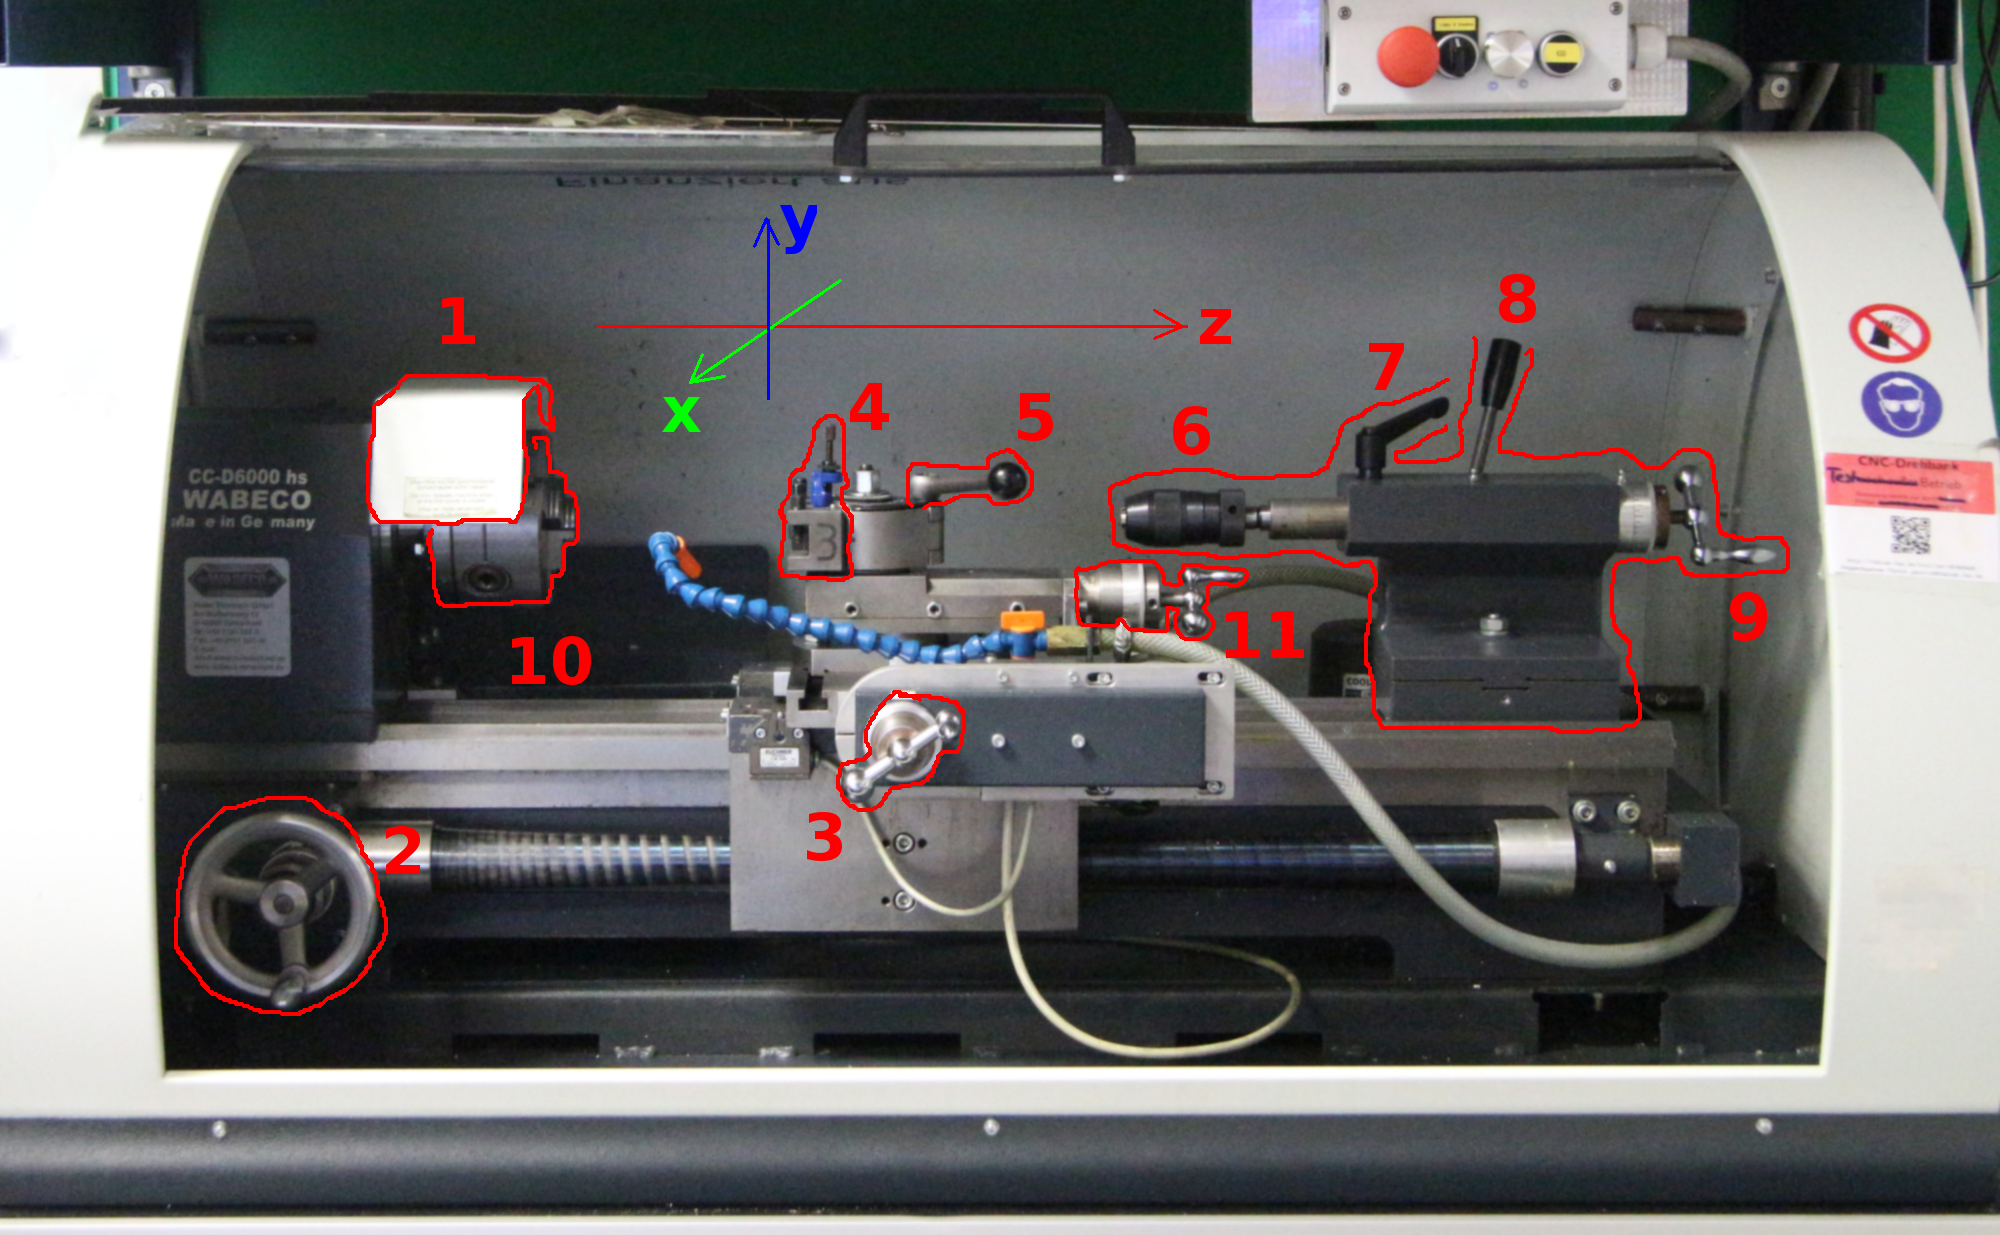
\includegraphics[width = 0.9\linewidth]{img/drehbank-uebersicht-beschreibung} \\
\caption{Das Koordinatensystem ist in diesem Bild oben mit den Pfeilspitzen in positiver Richtung eingezeichnet. Vorsicht: Der Koordinatenursprung ist einstellbar und gewöhnlich nicht an der eingezeichneten Stelle.}
\end{figure}


\subsection{Zentrierbohrung}
\label{handdrehen:zentrierbohrung}
Das Setzen einer Zentrierbohrung ist wichtig, um das Verlaufen des Bohrers beim Bohren zu verhindern
und das Gegenspannen des Werkstückes mit einer mitlaufenden Körnerspitze zu ermöglichen.
Bevor überhaupt eine Zentrierbohrung gesetzt werden kann ist die Fläche vorher wie in
Abschnitt \ref{handdrehen:Plandrehen} beschrieben plan zu drehen!

Die Bohrtiefe mit dem Zentrierbohrer muss so tief sein, dass die von der schrägen hinteren Fläche des Zentrierbohrers erzeugte Kontaktfläche zur mitlaufenden Körnerspitze gross genug ist. Eine zu kleine Kontaktfläche beschädigt die Körnerspitze.

Für die Zentrierbohrung ist der Zentrierbohrer ohne Klebeband zu verwenden.
Unbenutzte, neue Zentrierbohrer sind mit Klebeband markiert.

Falls das Bohrfutter nicht im Reitstock eingespannt ist, muss zunächst das dort montierte Werkzeug entfernt werden.
Dazu wird die Kurbel des Reitstockes soweit zurück gedreht, bis der  Kegel aus dem Reitstock gedrückt wird.
Dies kann etwas (aber nicht allzu viel) Kraft benötigen.
Manchmal hilft es auch ein wenig \enquote{Schwung} zu holen.

In die freie Kegelaufnahme des Reitstockes (sogenannte Reitstockpinole) wird dann das Bohrfutter eingeschoben.
Dazu muss die Pinole mindestens auf 15\,mm ausgefahren sein.
Unbedingt den sicheren Sitz des Werkzeuges prüfen!

\textbf{Unbedingt darauf achten, dass hierbei keinerlei Späne auf dem Bohrfutterkegel oder in der Reitstockaufnahme sind! Falls das Bohrfutter oder die mitlaufende Körnerspitze mit einem Span geklemmt wird, ist es sehr wahrscheinlich, dass sich weder das Futter noch die Spitze jemals wieder demontieren lassen ohne etwas ernsthaft zu beschädigen!}

Vorgehen:
\begin{itemize}
\item Zentrierbohrer einspannen
\item Reitstock bis an Material heran fahren und festklemmen
\item Richtige Drehzahl einstellen
\item Mit guter Handkraft bohren und immer wieder mit Öl schmieren!
\item Richtige Senkungstiefe beachten
\item Wenn die nötige Tiefe erreicht ist, Reitstockpinole zurück kurbeln

\end{itemize}

\subsection{Bohren}

Um das Verlaufen des Bohrers zu vermeiden ist es zunächst notwendig eine Zentrierbohrung wie im Kapitel \ref{handdrehen:zentrierbohrung} beschrieben anzubringen.
Anschließend bringt man das Bohrfutter an der Reitstockspindel an und wählt den passenden Bohrer aus.
Verwende hierfür unbedingt die Bohrer, die sich in der Schublade unter der Drehbank befinden, diese sind speziell reserviert um eine hohe Rundlaufgenauigkeit zu erhalten.

Positioniere den Bohrer kurz vor dem Werkstück und wähle die passende Drehzahl aus der Drehzahltabelle \todo{wo ist diese Drehzahltabelle?} an der Drehbank aus.
Danach kann durch Zustellung mit der Reitstockpinole gebohrt werden.
Dabei gilt wie bei jedem Bohrvorgang: Mit guter Handkraft bohren!
Ansonsten wird der Bohrer übermäßig verschlissen und die Qualität der Bohrung nimmt ab.

\subsection{Außendrehen} 

Das Außendrehen findet in der Regel in mehreren Bahnen mit dem richtigen Vorschub und Zustellung statt.
Hierbei wird grundsätzlich zum Futter hingearbeitet.
Es ist darauf zu achten auf keinen Fall mit dem Werkzeug ins Futter zu fahren, da ein solcher Crash Werkzeug und Maschine ernsthaft beschädigen und den Bediener schwer verletzen kann.
Am Ende ist in Richtung des Durchmessers vom Werkstück wegzufahren, bevor in Z-Richtung zum Beginn einer neuen Bahn gefahren wird.

\subsection{Innendrehen}

Das Innendrehen funktioniert im Grunde wie das Außendrehen. Es gibt jedoch trotzdem einige Besonderheiten:
\begin{itemize}
\item Anders als beim Außendrehen sieht man sein Werkzeug nur schlecht. Achte unbedingt darauf keine Kollision zu fahren.\\
\textbf{Nicht in die laufende Maschine beugen und versuchen so das Werkzeug zu sehen!}
\item Die Zustellung erfolgt beim Innendrehen in negativer Richtung, d.\,h. um 1\,mm abzunehmen ist mit dem Handrad 1\,mm zurückzufahren.
\end{itemize}

\subsection{Fasen}

Für das Anbringen von 45$^\circ$ Fasen gibt es ein spezielles Werkzeug, einen sogenannten Fasenmeißel.
Das Werkzeug ist gut an seiner blauen Lackierung und der breiten Schneide zu erkennen. 
\todo{Sobald Schnellspanner da und eingesetzt Werkzeugnummer anbringen, hier reinschreiben.}
Den Fasenmeißel spannt man senkrecht zum Werkstück ein, sodass die Schneide 45$^\circ$ zum Werkstück zeigt.
Danach kann an das Werkstück herangefahren werden und eine Fase angebracht werden.
Wenn sehr viele Fasen angebracht werden müssen, empfiehlt es sich nicht immer auf der selben Stelle der Schneide zu arbeiten.
Dies soll verhindern, dass die Schneide ungleichmäßig abgenutzt wird.

Für andere Winkel kann der Werkzeughalter mit dem Fasenmeißel auch verdreht in das Schnellspannfutter eingesetzt werden.

\subsection{Plan- und Runddrehen}
\label{handdrehen:Plandrehen}
\begin{wrapfigure}{r}{7.5cm}
\centering
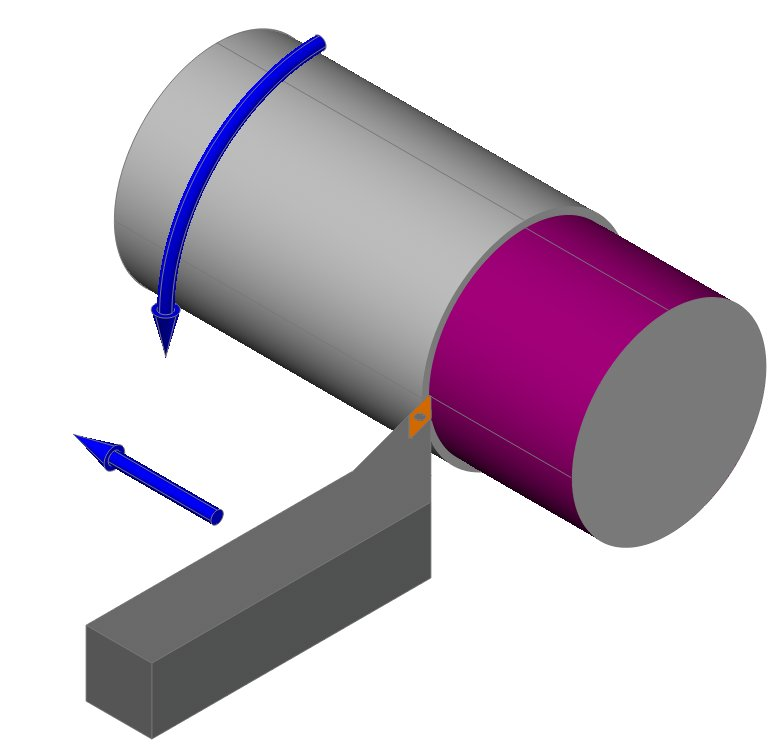
\includegraphics[height=3.4cm]{./img/laengs-rund-drehen.jpg}
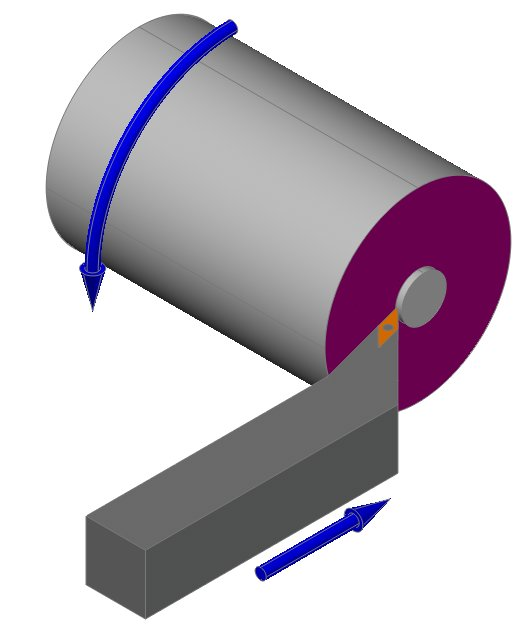
\includegraphics[height=3.4cm]{./img/quer-plan-drehen.jpg}
\caption{\href{https://commons.wikimedia.org/w/index.php?title=File:L\%C3\%A4ngs-Rund-Drehen.jpg&oldid=101538812}{Runddrehen}, \href{https://commons.wikimedia.org/w/index.php?title=File:Quer-Plan-Drehen.jpg&oldid=154429461}{Plandrehen}}
Autor: \href{https://commons.wikimedia.org/wiki/User:Florian_Schott}{Florian Schott}, Lizenz CC-BY-SA 3.0
\end{wrapfigure}

Zum Runddrehen (längs) wird mit konstantem X für eine radiale Aussenfläche abgedreht.
Beim Plandrehen wird hingegen bei konstantem Z eine Stirnfläche abgedreht. 

Beim Plandrehen wird auch ein normaler Außendrehmeißel verwendet, jedoch mit der sonst nicht genutzten hinteren Schneide. Dabei darf man sich nicht in X-Richtung über die Drehachse hinaus bewegen, da hinter der Drehachse das Material den Meißel von der falschen Seite anläuft.

Das Abdrehen einer radialen oder Stirnfläche kann auch zum Setzen von Nullpunkten mitverwendet werden, wenn man die \enquote{Antasten}-Funktion der Steuersoftware bei unveränderter anzutastender Koordinate verwendet.

\subsection{Abstechen}
Beim Abstechen wird das Werkstück an einer Stelle durchtrennt. Abstechen ist eine vergleichsweise gefährliche Operation.

Alternativ zum Abstechen kann das Teil eventuell nur \enquote{angestochen} werden. Den Rest kann man dann außerhalb der Drehbank mit einer Säge trennen und anschließend die Schnittfläche abschleifen oder plan drehen.

\subsubsection{Gefahren beim Abstechen}
\textbf{Der abgestochene Werkstückteil kann bei hoher Drehzahl aus der Maschine springen und den Bediener schwer verletzen!} Dies kann insbesondere bei schweren oder langen Teilen vorkommen. Diese springen durch den Restdrehimpuls, rollen oder knicken ab und werden durch die Drehbeweggung \enquote{geworfen}.

\textbf{Gegengespannten Werkstücke können sich beim Abstechen verklemmen.} Dies kommt zum einen daher, dass die Körnerspitze gefedert ist. Daher ist ggf. die Körnerspitze leicht zu lockern. Zum anderen kann allein durch die Geometrie das Werkstück sich beim Herunterfallen zwischen Körnerspitze, Werkzeug und drehendem Werkstückteil verklemmen und unkontrolliert durch die Maschine springen.

Es ist also immer sorgfältig abzuwägen, ob ein Abstechen sicher möglich ist.

Eine niedrige Spindeldrehzahl senkt die Gefahren. Dafür kann auch eine nicht-optimale niedrigere Schnittgeschwindigkeit in Kauf genommen werden.


\subsubsection{Durchführung}
Für ein Abstechen wird der Stechmeißel benötigt. Dieser wird 90$^\circ$ zum Werkstück eingespannt.
Es wird zu Beginn langsamer zum Ende hin schneller möglichst nahe am Futter abgestochen.

\todo{erklären, wieso schneller -- ist die Drehzahl gemeint?}

Außerdem ist es sinnvoll nicht kontinuierlich zu schneiden, sondern immer wieder mit Unterbrechungen einen Span abzunehmen.
Dabei zügig aus dem Werkstück herausfahren, sonst kann sich das Werkzeug aufgrund von Wärmedehnung mit dem Werkstück verklemmen!

Während des Schnittvorganges immer wieder mit Öl schmieren.

\textbf{Greife niemals in die drehende Maschine, um das abgestochene Bauteil zu entnehmen! Vorher Spindel ausschalten!}





\subsection{Gegenspannen}
\label{handdrehen:gegenspannen}

Vorgehen:
\begin{itemize}
\item Zunächst Zentrierbohrung (\ref{handdrehen:zentrierbohrung}) setzen\\
	\textbf{WICHTIG: eine gute Zentrierbohrung mit sauberen Flanken im richtigen Winkel ist essentiell, ansonsten überhitzt die Spitze der Körnerspitze, da Gleitreibung statt Haftreibung auftritt (die Körnerspitze dreht nicht sauber mit). Im Zweifelsfall nochmal mit dem Zentrierbohrer nachbesseren, falls die Spitze nicht sauber mitläuft.} 
\item Sicherstellen, dass alle Späne aus der Bohrung entfernt sind
\item Falls nicht die mitlaufende Körnerspitze montiert ist, Bohrfutter o.\,Ä. aus dem Reitstock entfernen
\item Körnerspitze mit leichtem Druck in die Reitstockpinole einsetzen\\
\textbf{Unbedingt auf Spanfreiheit achten! siehe \ref{handdrehen:zentrierbohrung}}
\item Klemmung des Reitstock öffnen und Körnerspitze bis kurz vor Materialkontakt schieben 
\item Klemmung schließen
\item Reitstockpinole ausfahren bis Körnerspitze am Werkstück anliegt.\\
\textbf{WICHTIG: Auf keinen Fall zu fest spannen! Bei der Bearbeitung dehnt sich das Material aus. Wird mit zu viel Kraft gegengespannt, verbrennen die Lager der Körnerspitze}
\item Reitstockpinole mit dem Hebel auf der Oberseite arretieren
\item Spindel starten und langsam die Drehzahl erhöhen; wenn die Körnerspitze nicht sauber mitläuft muss nochmal zentriert werden
\end{itemize}

\subsection{Schleifen und Polieren}
Schleifen mit Schleifpapierband durch Umschlingen ist verboten!
Schleifen darf nur mit einem speziell dafür vorgesehenen Werkzeug durchgeführt werden. Die Verwendung anderer Werkzeuge wie Feilen ist nicht gestattet, da diese vom Futter oder vom Werkstück erfasst werden können und den Bediener schwer verletzen.

\subsection{Nut drehen}

Das Vorgehen entspricht der Vorgehensweise beim Abstechen.
Als Werkzeug wird eine Stechwendeschneidplatte (sternförmig), Werkzeug Nummer 4, verwendet.

% die folgende Erklärung ist zu gefährlich:
%\subsection{Oberflächen-schonend Spannen} \textbf{WICHTIG: Wenn du keine ausreichende Erfahrung hast frage dabei IMMER einen erfahrenen Betreuer, der an der Drehbank eingewiesen ist. Ein unzuverlässig gespanntes Werkstück ist lebensgefährlich!}\\ Eine Möglichkeit ist zwischen dem Werkstück und dem Futter ein Stück grobes Schmirgelpapier (Körnung 80 o.Ä) einzulegen, dass das Werkstück komplett umschlingt. Dabei zeigt die raue Seite nach außen zum Futter. Das Schmirgelpapier sollte dabei möglichst nicht überlappen. Außerdem muss mit einer Messuhr der Rundlauf überprüft werden und notfalls durch ein Ausrichten des Werkstückes korrigiert werden. Problem ist nämlich, dass das Schmirgelpapier, das die Reibung erhöht leider auch die Ausrichtung des Werkstückes zu den Spannbolzen behindert. Das Einspannen mit Schmirgelpapier empfiehlt sich vor allem bei einem Spannen auf Gewinden.

\subsection{Rändeln}
\label{handdrehen:raendeln}

Rändeln ist das Einprägen von Mustern in das Werkstück, beispielsweise um geriffelte Grifflächen an Stellschrauben zu erzeugen.

Zur Zeit ist nur manuelles Rändeln für Alu möglich. Überschneidungen des Rändels nur sehr schwer vermeidbar, daher sieht es nicht optimal aus, aber besser als nichts.
\todoUnwichtig{CNC-Rändeln in Arbeit}

Es ist ein relativ preiswertes Rändelwerkzeug vorhanden.
Das Werkzeug kann in den Schnellspannhalter des Fasenmeißels gespannt werden.
Es besteht aus einem einspannbaren Körper mit einem flexiblem, mit zwei Rändelrädern ausgestatteten Kopf.

Die Verwendung ist relativ simpel.
Sobald das Werkstück fertig bearbeitet ist, kann gerändelt werden.
Dazu muss es möglichst kurz gespannt werden (Rändeln ist das kraftintensivste Drehverfahren!)

Zur Vorbereitung die \enquote{Lager} des Rändelwerkzeuges gut ölen.
Etwas Kühlschmierstoff oder Öl auf den Laufflächen schadet auch nicht. 
Nun wird das Rändelwerkzeug so nahe an das Werkstück gefahren, dass der flexible Kopf locker auf das Werkstück gelegt werden kann.
Danach befindet sich das Werkstück zwischen den beiden Rändelrollen.

Nun wird eine mittlere Drehzahl eingestellt und Rechtslauf aktiviert. 
Das Rändelwerkzeug wird langsam im Randbereich des gewünschten Rändels an das Werkstück gefahren. 
Bei schwer spanbaren Materialien empfiehlt es sich zunächst nur die Hälfte der Rollen zu belasten, um die auftretenden Kräfte gering zu halten.

Je nach Material wird nun $1$\,mm zugestellt. Sobald die Rollen anfangen zu schneiden, darf das Werkzeug nicht mehr von der Oberfläche getrennt werden, um Überschneidungen im Rändel zu vermeiden.
Um einen sauberen Rändel zu erzeugen, sollte die Rändelrolle mit wohl dosiertem Druck gleichmäßig über die Oberfläche geführt werden.
Um mögliche Späne während des Rändelns abzuspülen empfielt es sich immer wieder mit einem Schwung KSS die Laufflächen zu spülen.
Zwischendurch kann die Maschine abgeschalten werden, um zu überprüfen, ob der Anpressdruck ausreicht.
Für das Ergebnis in Grafik \ref{fig:raendel} wurde im Anschluss an das Rändeln noch angefast.
Der Rändel in der Grafik ist überschnitten, da die Maschine nicht schnell genug verfahren wurde.

\begin{figure}[hb]
\caption{gerändeltes Stück Aluminium}
%Autor: Patrick Kanzler, Public Domain, 2014
\label{fig:raendel}
\centering
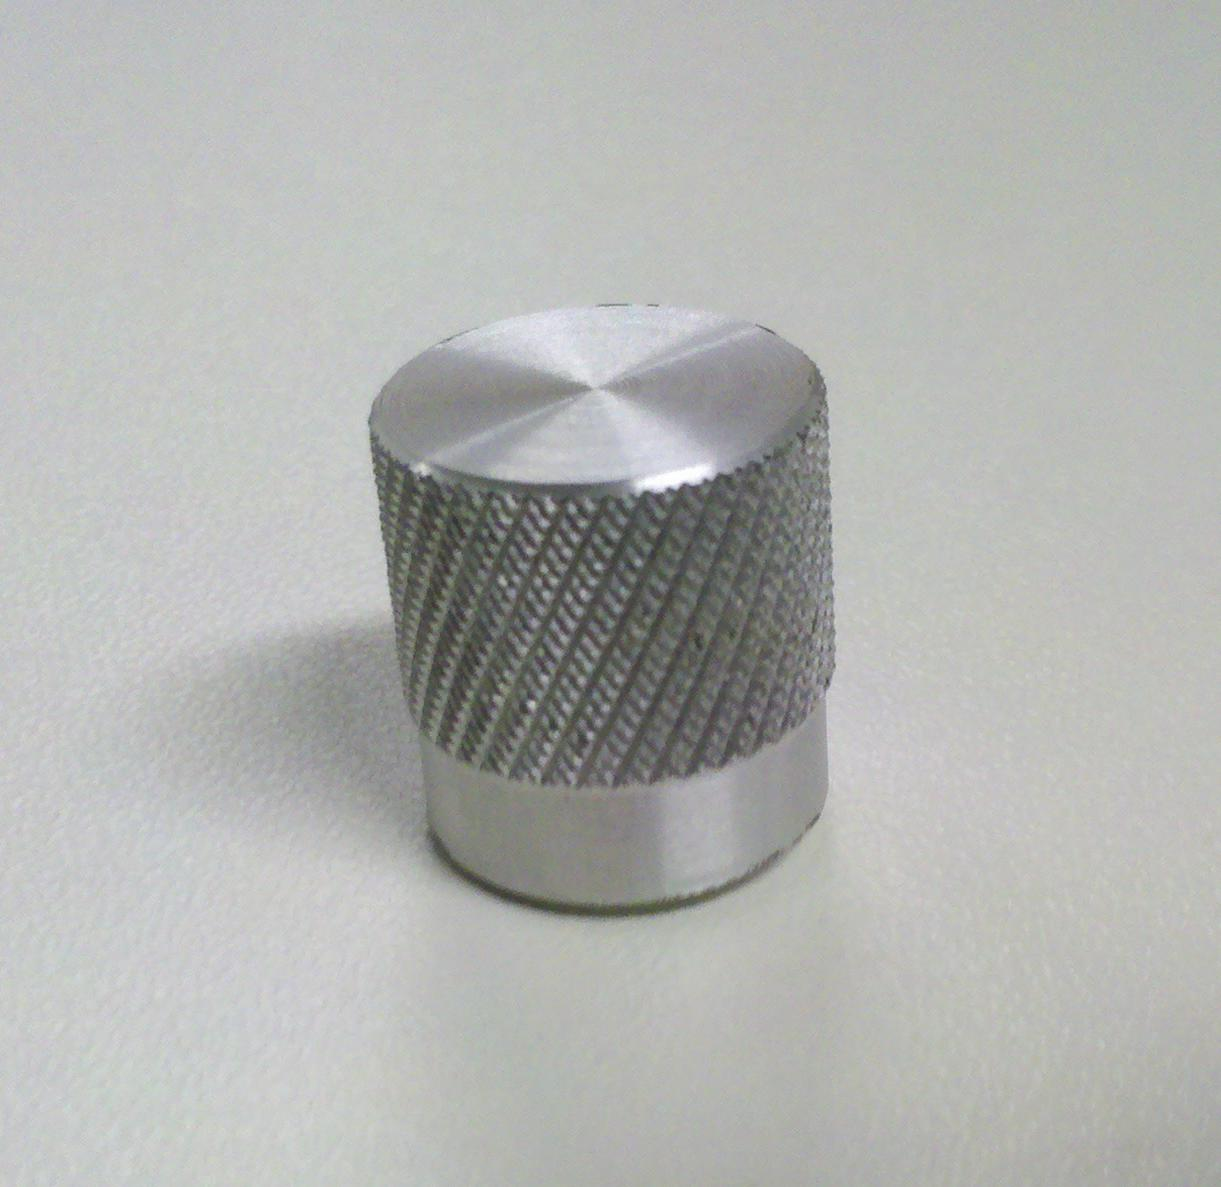
\includegraphics[width=.5\linewidth]{img/raendel}
\end{figure}
\newpage
\section{CNC - Drehen}

Beim CNC-Drehen wird die Drehmaschine durch ein in GCode geschriebenes oder automatisch aus einer CAM-Anwendung wie NX erzeugtes Programm gesteuert.

Voraussetzungen für eine Erstellung des GCode aus NX sind:
\begin{itemize}
	\item Ein dreidimensionales Modell des rotationssymmetrischen Werkstückes.
	\item Ein dreidimensionales Modell des Rohstückes.
	\item Daten der vorhandenen Werkzeuge und der Maschine.
\end{itemize}
Diese können in der Konstruktionsanwendung in NX erzeugt werden.

In der Fertigungsanwendung wird hieraus dann ein Arbeitsablauf erstellt, der simuliert und in GCode ausgegeben werden kann.

\subsection{Job-Vorbereitung mit NX}
Diese Einweisung wurde mit NX 9 erstellt. Möglicherweise kann das hier geschilderte Verhalten in anderen Versionen, Sprachen oder Installationen abweichen. NX enthält generell einige Fehler und Übersetzungsfehler sowie schwer verständliche Terminologie. Ein denkender Bediener wird generell bei allen Beschreibungen dieses Dokuments vorausgesetzt.

NX wird in mehreren Tutorials erklärt. Diese sind über die Hilfefunktion in der Fertigungs-Anwendung auffindbar. Hierbei ist insbesondere das speziell für das Drehen vorgesehene Tutorial als Einstieg sehr zu empfehlen. Auf im Tutorial vorkommende Sachverhalte wird hier nicht mehr gesondert eingegangen, dieser Abschnitt beschreibt nur die Besonderheiten im Falle des FabLab.

\todoUnwichtig{Diese Abschnitte beschreiben vorerst nur die gröbsten Fallstricke.} Weitere Informationen findest du in der Kurzanleitung: \url{https://github.com/fau-fablab/NX9-linuxcnc-lathe-PP/blob/master/Anleitung%20NX%20Drehen.txt}
\todo{diese anleitung NX drehen aus postprozessor repo hier hinein mergen, zumindest die crash-kritischen sachen}

\subsubsection{Werkzeuge}

Die im FabLab vorhandenen Drehwerkzeuge sind vermessen und in LinuxCNC unter der auf dem Schnellwechelhalter vorhandenen Nummer eingetragen. Es ist unbedingt darauf zu achten, dass bei der Verwendung von Werkzeugen in NX auch die richtige Werkzeugnummer verwendet wird, da hierueber die Positionskorrektur ausgewählt wird.

Die Werkzeugbibliothek von NX enthält die im FabLab vorhandenen Werkzeuge mit bereits richtig voreingestellten Eigenschaften und Abmessungen. \todo{Auffinden dieser Werkzeuge? Bezeichnungsschema?}

\todo{Laden der Werkzeugbibliothek?}

\todo{gespiegelte Anzeige oder nicht? bisher widersprüchliche Informationen und verschiedene Ansätze (arw/Toni/Max), höchstwahrscheinlich sogar inkonsistent zu Maxs Online-Kurzanleitung}


\subsubsection{Simulation}

NX bietet die Möglichkeit Arbeitsabläufe einer Fertigung zu simulieren. Damit sollte man die Kollisionsfreiheit von Programmen prüfen. Achtung: NX hat diverse Bugs bei der Simulationsanzeige, Abhilfe schafft eine langsamere Ablaufgeschwindigkeit, das Wechseln der Tabs in der Simulationssteuerung oder ein Ein- und Ausblenden des 3D-Modells des Werkzeugs.

\subsubsection{Start- und Endpunkte}


\todo{Containment (wie auch immer das auf deutsch heißt) erklären, auch Anfahrbewegungen an Operation}

Es \textbf{müssen} für jede Operation Start- und Endpunkte in ausreichend grossem Abstand vom Rohmaterial gewählt sowie passende Anfahrbewegungen vorgegeben werden. Die Punkte sollten sich immer nahe beieinander befinden, da später LinuxCNC beim Programmwechsel einen Pfad zwischen vorherigem End- und nächstem Startpunkt fahren wird, ohne dass dies auf Kollisionen prüfbar ist.
Die Bewegung in der Simulation nur als Sprung gezeigt und erfolgt ausserdem mit der maximalen Geschwindigkeit \texttt{G0}.

Nähere Informationen dazu finden sich vorerst nur in der NX-Kurzanleitung \url{https://github.com/fau-fablab/NX9-linuxcnc-lathe-PP/blob/master/Anleitung%20NX%20Drehen.txt}.
\todo{Containment, Anfahrbewegungen hier erklären}

\subsubsection{Postprocessing}

Die Endgültige Erzeugung von GCode erfolgt im "`Postprocessing"' genannten Arbeitsschritt. Hierzu wird ein für die im FabLab verwendete Maschine erstelltes Postprocessing-Programm verwendet. \todo{Beschreibung Auswahl postprocessing}

Es ist sinnvoll nach dem Postprocessing NX und alle Ordner die die ausgegebenen
GCode-Dateien verwenden zu schliessen, da es sonst zu Locking-Problemen und
somit zu mysteriös verschwindenden, nicht-löschbaren oder ähnlich
"`interessanten"' Dateien kommt. Ausserdem ist ein neuer Ordner pro neuer
Version der GCode-Ausgabe sinnvoll.

Momentan ist aufgrund von Beschränkungen im Postprocessing nur ein Werkzeug pro GCode-Datei möglich, ein Werkzeugwechsel, der nicht am Anfang sondern Mitten im Ablauf der Datei stattfindet wird nicht unterstützt. Daher sind für verschiedene Werkzeuge verschiedene Dateien zu erstellen.

\subsection{Bedienung von LinuxCNC}

Zur Ausführung von vorhandenem GCode sind die folgenen Schritte der Reihe nach auszuführen.

\subsubsection{Einschalten}
Die Einschaltreihenfolge ist:
\begin{itemize}
	\item Steuerrechner einschalten
	\item Drehmaschine am Hauptschalter einschalten
	\item Drehmaschine auf Betriebsart \enquote{Auto} stellen
	\item LinuxCNC auf dem Steuerrechner starten
	\item Mit dem Not-Aus-Reset den Not-Aus freigeben
	\item 2. Icon in LinuxCNC "`Maschine an/aus (F2)"' drücken (die Maschine läuft hier noch nicht an, die Bezeichnung ist leicht verwirrend)
\end{itemize}

\subsubsection{Nullpunkt und Referenzierung}

Zunächst muss eine Referenzfahrt der Maschine durchgeführt werden. Hierzu ohne eingelegtes Material und ohne Werkzeug den LinuxCNC-Knopf \enquote{Referenzfahrt} betätigen. Hierzu muss die Schutzhaube geschlossen sein. Die Maschine fährt nun bis zu den mit Endschaltern versehenen Positionen in beiden Achsen.

Die Einstellung des Nullpunkts des Koordinatensystems hängt vom im GCode angenommenen Nullpunkt ab. Beispielsweise kann der Nullpunkt der Z-Achse am rechten oder linken Ende des Werkstücks liegen, der Nullpunkt der X-Achse muss in der Drehachse\footnote{Wird nicht die Drehachse als X-Nullpunkt gewählt, funktioniert die Steuerung der Drehzahl für die konstante Schnittgeschwindigkeit nicht.} liegen. Bei der Erstellung des GCode sollte die Wahl des Nullpunkts daher separat vermerkt werden.

Das Werkzeug Nummer 3 ist das Referenzwerkzeug, d.h. die X- und Z-Offsets des Koordinatensystems sind bei diesem Werkzeug exakt $0$, alle anderen Werkzeuge sind darauf abgestimmt. Daher ist es sinnvoll, den Nullpunkt mithilfe von Werkzeug 3 zu setzen. Hierzu geht man wie folgt vor:
\begin{itemize}
	\item Rohteil wie weiter oben beschrieben einspannen
	\item Durchmesser des Rohteils mit Schieblehre bestimmen, Radius berechnen
	\item Werkzeug 3 einsetzen\footnote{Es ist auch möglich ein anderes Werkzeug als Werkzeug 3 zum Setzen des Nullpunktes zu verwenden. Hierzu müssen aber zuerst die Werkzeugoffsets dieses anderen Werkzeugs geladen werden. Hierzu muss man manuell in der Registerkarte \enquote{MDI (F5)} den GCode \texttt{M6 T$n$} wobei $n$ die Werkzeugnummer ist, also beispielsweise \texttt{M6 T2} für Werkzeug Nummer 2 eingeben. Anschliessend muss noch \texttt{G43} eingegeben werden um das Koordinatensystem dem gerade gesetzten Werkzeug anzupassen. Nach dem Rückwechsel auf die Registerkarte \enquote{Manuelle Kontrolle (F3)} kann man in der Anleitung normal weiter fortfahren. Es ist zu beachten, dass sich nicht alle Werkzeuge aufgrund ihrer Geometrie zur Nullpunktseinstellung eignen.}
	\item Schutzhaube schliessen
	\item Spindel im Rechtslauf drehen lassen, Drehzahl grösser 1000 Umdrehungen (Einstellung mit \enquote{+} und \enquote{-}, Drehzahlanzeige ist grüner Balkengraph rechts oben)
	\item Schrittgeschwindigkeit langsam einstellen, z.B. $20\,\frac{\mathrm{mm}}{\mathrm{min}}$
	\item mit Pfeiltasten kann das Werkzeug verfahren werden
	\item mit dem Werkzeug die Aussenfläche (aussen auf der Rundung) leicht berühren, so dass gerade so ein minimaler Span auftritt, Werkzeug an dieser Position \textbf{stehenlassen}
	\item mittels \enquote{Antasten} kann nun die Werkzeugposition spezifiziert werden, hierbei für die Aussenfläche die X-Achse im erscheinenden Dialog auswählen und den oben vermessenen Radius als X-Koordinate angeben
	\item der Nullpunkt der X-Achse ist nun die Rotationsachse
	\item mit der \enquote{nach-unten-Taste} von der Aussenflaeche des Rohteils wegfahren.
	\item die Stirnfläche kann in gleicher Weise angefahren werden um den Nullpunkt der Z-Achse zu setzen, mit dem im Antasten-Dialog angegebenen Wert kann bestimmt werden ob der Nullpunkt dabei an der Stirnseite oder an anderer Stelle liegen soll.
	\item wiederum in Richtung der Z-Achse vom Rohteil wegfahren bevor Bewegungen in der X-Achse durchgeführt werden
	\item Spindel mit dem \enquote{Stop}-Knopf anhalten. Bei Stillstand kann die Schutzhaube wieder geöffnet werden.
\end{itemize}

\todo{Verfolgungspunkt aller Werkzeuge beschreiben}

Analog kann auch das Rohteil hier abgedreht werden und dabei der Nullpunkt festgelegt oder verstellt werden. Die obige Anleitung ist zweckmässig modifiziert zu verwenden je nach Wahl des Nullpunktes im GCode. Wird der Nullpunkt falsch gewählt sind Kollisionen, schwere Schäden und Unfälle möglich.

\subsubsection{Laden und Kontrollieren des Jobs}

Mit der \enquote{Datei öffnen}-Funktion kann der GCode geöffnet werden. Die im GCode enthaltenen Fahrpfade werden angezeigt, diese können nun geprüft werden. Dazu kann man:
\begin{itemize}
	\item die Pfade anschauen, dazu ggf. mit dem Besen-Icon vorherige Fahrpfade löschen
	\item Mit eingesetztem Werkzeug in manueller Fahrt (Pfeiltasten) können visuell die Grenzen der Fahrpfade \enquote{erforscht} werden. Achtung: Hierbei keinesfalls mit dem Werkzeug ein Maschinenteil oder das Rohteil berühren, selbst leichtes Anfahren kann z.B. die Schneidplatten beschädigen.
	\item Einen Leerlauf des Programms ohne Werkzeug durchführen. Achtung: Bei sehr groben Fehlern kann hier zwar nicht das Werkzeug, aber der Halter kollidieren! Man kann auch durch geeignete Wahl des Z-Nullpunktes die Leerfahrt weiter \enquote{rechts} in grossem Abstand zur Spindel durchführen.
\end{itemize}

Ein Leerlauf ohne Werkzeug ist auch zum Einüben des Arbeitsablaufs sinnvoll.

\subsubsection{Jobablauf}

Ein Job wird durch Drücken des \enquote{Start}-Icons gestartet. Vorher sollte darauf geachtet werden,
dass das passende Werkzeug eingelegt ist. LinuxCNC wird bei den meisten Jobs zum Start des Programms nach einem Werkzeugwechsel fragen. Bei GCode der nicht mit NX und dem FabLab-Preprocessing-Skript erzeugt wurde muss das aber nicht unbedingt der Fall sein.

KSS ist manuell am Schaltschrank einzuschalten, es geht noch nicht automatisch.
\todoUnwichtig{Text ändern, sobald es automatisch geht}

Der Job kann mit den entsprechenden Icons pausiert oder angehalten werden. Beim Werkzeugwechsel ist ggf. auch eine Pausierung mit dem entsprechenden Knopf aufzuheben.

Im Programmablauf muss die Schutzhaube geschlossen sein. Die einzige Ausnahme davon ist wenn LinuxCNC einen Werkzeugwechsel anfordert. Die Maschine muss beim Programmablauf unbedingt genau beobachtet werden um ggf. rechtzeitig den Not-Aus-Schalter betätigen zu können falls Kollissionen oder andere Probleme auftreten. Bei \enquote{harmloseren} Problemen ist das Stop-Icon oder die Taste \enquote{Esc} ebenfalls geeignet.

Nach Ablauf des Jobs bis zum Stillstand der Spindel warten, bevor die Schutzhaube geöffnet wird.

Besteht ein Job aus mehreren GCode-Dateien, weil beispielsweise mehrere Werkzeugwechsel notwendig sind kann nun mit dem Laden der nächsten Datei fortgefahren werden.

\newpage
\section{Aufräumen und Wartung}


\subsection{Aufräumen und Wartung}
Nach dem Drehen:

\begin{itemize}
 \item Späne wegräumen (aufsammeln/aufkehren), soweit man vernünftig hinkommt. Auf jeden Fall frei sein muss der vordere Bereich rund um die Handräder sowie der Bereich neben den Endschaltern.
 \item Rest wegsaugen, wenn kein Kühlschmiersiff ist. Der Staubsauger mag keinen Siff (gammelt) und keine langen Späne (verstopfen den Saugschlauch).
 \item Drehmeißel außerhalb der Bank ausblasen, Spitzen der Platten auf Beschädigung oder Verfärbung kontrollieren
 \item Drehmeißel wegräumen, keinen im Schnellwechsler gespannt stehen lassen, entspannt ist ok.
 \item Alle Teile haben in der Schublade unter der Drehbank ihren Platz, wo sie auch wieder hingehören! Der Futterschlüssel gehört an den Magneten ganz links in der Schutzhaube.
\end{itemize}


Alu- und POM-Späne nicht mischen. Wir können nur rein-Alu-Späne bei der MEW abgeben! Alles andere ist Mischmüll. (Außer teure Metalle aka. Messing/Silber/Blei/Inconel90, diese extra und sortenrein aufbewahren)

\appendix

\section{Quellen}
\begin{itemize}
 \item \href{http://publikationen.dguv.de/dguv/pdf/10002/bgi578.pdf}{BGI 578 Sicherheit durch Betriebsanweisungen}
 \item \href{http://www.arbeitssicherheit.de/media/pdfs/CCC_1290.pdf}{BGI 2003 Maschinen der Zerspanung}
 \item BGV Muster-Betriebsanweisung Drehmaschinen
\end{itemize}

\todo{Copyright anpassen... Betriebsanweisung ausnehmen?}
% \ccLicense{drehbank-einweisung}{Einweisung Drehbank}

\end{document}
